\chapter{Многоканальная система в форме вход-состояние-выход}
\label{ch:chap4}

\section{Строим структурную схему}

В этом задании мы будем рассматривать систему следующего вида: 
 $$
    \begin{cases}
        x =Ax+Bu,\\
        y = Cx.
    \end{cases}
$$

С учётом моих коэффициентов она превратится в:
$$
\begin{cases}
    \feqvector{\dot{x_1},\dot{x_2}} = \begin{bmatrix}
        0 & -2  \\
        1 & -3 
        \end{bmatrix} \feqvector{x_1,x_2} + \begin{bmatrix}
            2 & 3  \\
            3 & 5 
            \end{bmatrix} \feqvector{u_1,u_2},\\
    y = \begin{bmatrix}
        3 & 5  \\
        4 & 7 
        \end{bmatrix} \feqvector{x_1,x_2}.
\end{cases}
$$

Для удобства построения схемы, перемножим элементы системы и выпишем их:
$$
\begin{aligned}
    \dot{x_1} = -2x_2 + u_1 + 3u_2 \\
    \dot{x_2} = x_1 - 3x_2 + 3u_1 +5u_2 \\
    y_1 = 3x_1 +5x_2 \\
    y_2 = 4x_1 + 7x_2
\end{aligned}
$$
Теперь построить схему стало значительно проще, вот же она:
\begin{figure}[ht]
    \centering
    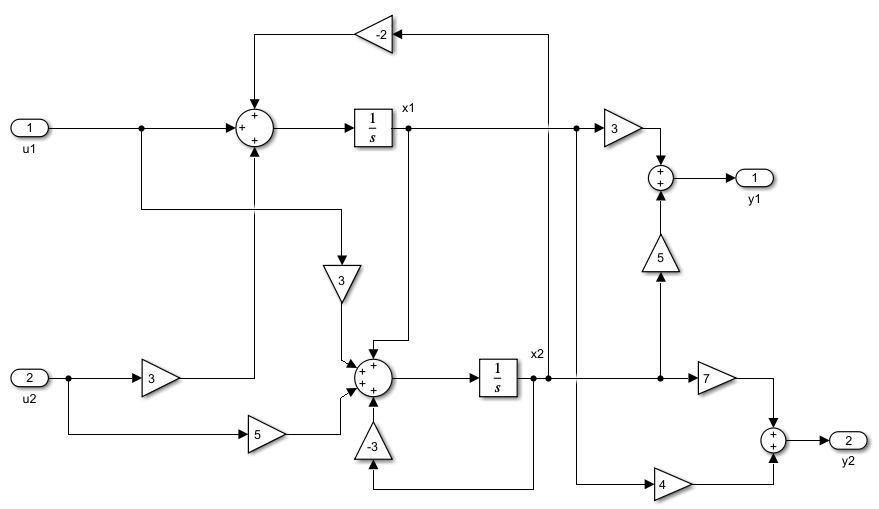
\includegraphics[width=1\textwidth]{scheme_task3_multiple_ECE.png}
  \caption{Схему - MIMO, ECE}
  \end{figure}

\section{Моделируем}

\begin{figure}[h]
	\begin{subfigure}{0.5\textwidth}
		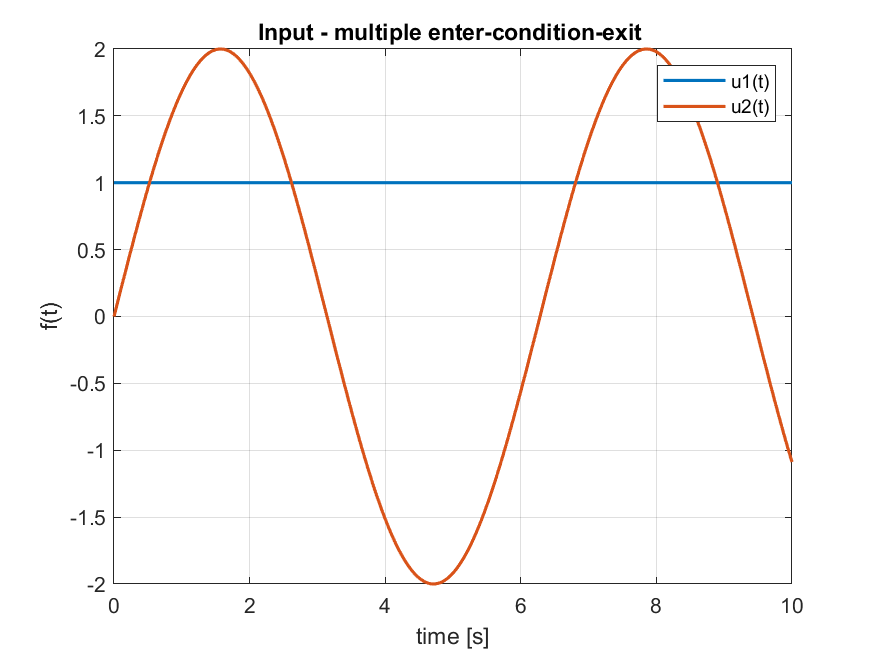
\includegraphics[width=0.9\linewidth, height=6cm]{input_task3_multiple_ECE.png} 
	\end{subfigure}
	\begin{subfigure}{0.5\textwidth}
		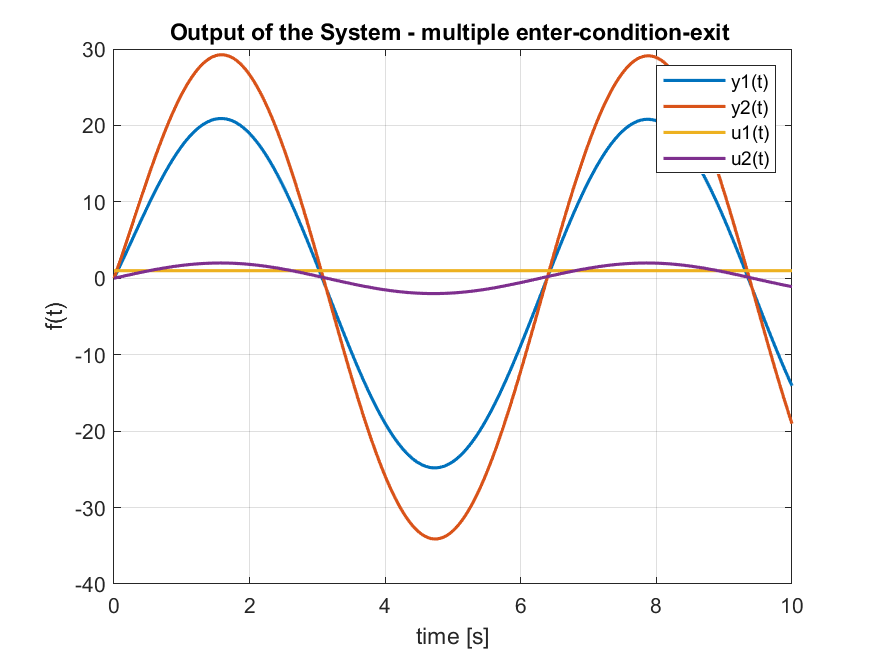
\includegraphics[width=0.9\linewidth, height=6cm]{output_task3_multiple_ECE.png}
	\end{subfigure}
	\caption{Симуляция - $u_1(t) = 1 , u_2(t) = 2sin(t)$}
\end{figure}

\endinput